\documentclass[12pt,a4paper]{article}
\usepackage[utf8]{inputenc}
\usepackage[T1]{fontenc}
\usepackage{amsmath}
\usepackage{amsfonts}
\usepackage{amssymb}
\usepackage{graphicx}
\usepackage{tikz}
\usepackage{titlecaps}
\usepackage{float}
\usepackage{setspace}
\usepackage{wrapfig}

\usepackage[french]{nomencl}
\usepackage{french}
\usepackage{listings}
\usepackage{verbatim}
\usepackage[hidelinks]{hyperref}
\usepackage{pdfpages}
\usepackage{fancyhdr}

\usepackage{color}
\definecolor{lightgray}{rgb}{.9,.9,.9}
\definecolor{darkgray}{rgb}{.4,.4,.4}
\definecolor{purple}{rgb}{0.65, 0.12, 0.82}

\lstdefinelanguage{JavaScript}{
	keywords={typeof, new, true, false, catch, function, return, null, catch, switch, var, if, in, while, do, else, case, break},
	keywordstyle=\color{blue}\bfseries,
	ndkeywords={class, export, boolean, throw, implements, import, this},
	ndkeywordstyle=\color{darkgray}\bfseries,
	identifierstyle=\color{black},
	sensitive=false,
	comment=[l]{//},
	morecomment=[s]{/*}{*/},
	commentstyle=\color{purple}\ttfamily,
	stringstyle=\color{red}\ttfamily,
	morestring=[b]',
	morestring=[b]"
}

\lstset{
	language=SQL,
	backgroundcolor=\color{lightgray},
	extendedchars=true,
	basicstyle=\footnotesize\ttfamily,
	showstringspaces=false,
	showspaces=false,
	numbers=left,
	numberstyle=\footnotesize,
	numbersep=9pt,
	tabsize=2,
	breaklines=true,
	showtabs=false,
	captionpos=b
}


\author{
	Boubekri, Abdelmalek \     \texttt{abdelmalek.boubekri@etu.univ-rouen.fr}
	\and
	Mezheri, Bilal\   		   \texttt{bilal.mezheri@etu.univ-rouen.fr}
}


\title{	Université de Rouen, UFR Sciences et Techniques\\
		Master 1 IGIS – Bases de données\\
		Gestion des patients et des traitements\\ }




\begin{document}
	
	\maketitle
	\newpage
	
	\tableofcontents
	\makenomenclature
	\printnomenclature


\section{Contexte}


Le but de l’application est de gérer des patients qui suivent des traitements
prescrits par des médecins suite à des observations faites lors de consultations.
Un traitement a une durée et est constitué de médicaments.

Un médicament possède plusieurs caractéristiques. Notamment : les indications, contre-indications, des substances actives, des effets indésirables connus, disponibles dans des notices.

Une substance active peut générer des effets indésirables.

Deux médicaments pris simultanément peuvent provoquer des interactions médicamenteuses.
Les maladies, substances actives, les effets indésirables sont organisés de manière hiérarchique avec héritage des propriétés.

Un patient a également des caractéristiques et peut souffrir d’une maladie chronique qui nécessite un traitement de longue durée.

Un médecin peut travailler pour un laboratoire pharmaceutique et peut également développer un médicament.

\subsection{Règles métier du système d'information}
les règles de gestion sont décrites ci-dessous:

\begin{enumerate}

\item Un patient peut consulter un médecin;
\item Une maladie a plusieurs symptômes;
\item Durant une consultation, plusieurs symptômes peuvent être observés;
\item On peut traiter une maladie avec un traitement;
\item Un médicament peut être développé par un laboratoire et plusieurs médecins;
\item Un médicament a une notice;
\item Une notice contient des indication, contre-indications et des substances actives;
\item Une substance active peut avoir plusieurs effets indésirables;
\item Une substance active peut interagir avec une autre substance active;
\item 

\end{enumerate}


Après avoir pris connaissance des exigences, on doit suivre les étapes suivantes afin de concrétiser la base de données.

\begin{itemize}

\item Modélisation E/A avec l'outil open-source Dia;
\item Transformation au modèle relationnel ;
\item Implémentation de la Base de données en PL/SQL via Oracle-xe-11g.

\end{itemize}


\section{Modélisation}
\subsection{Modèle entité association}

\begin{figure}[H]
	\centering
	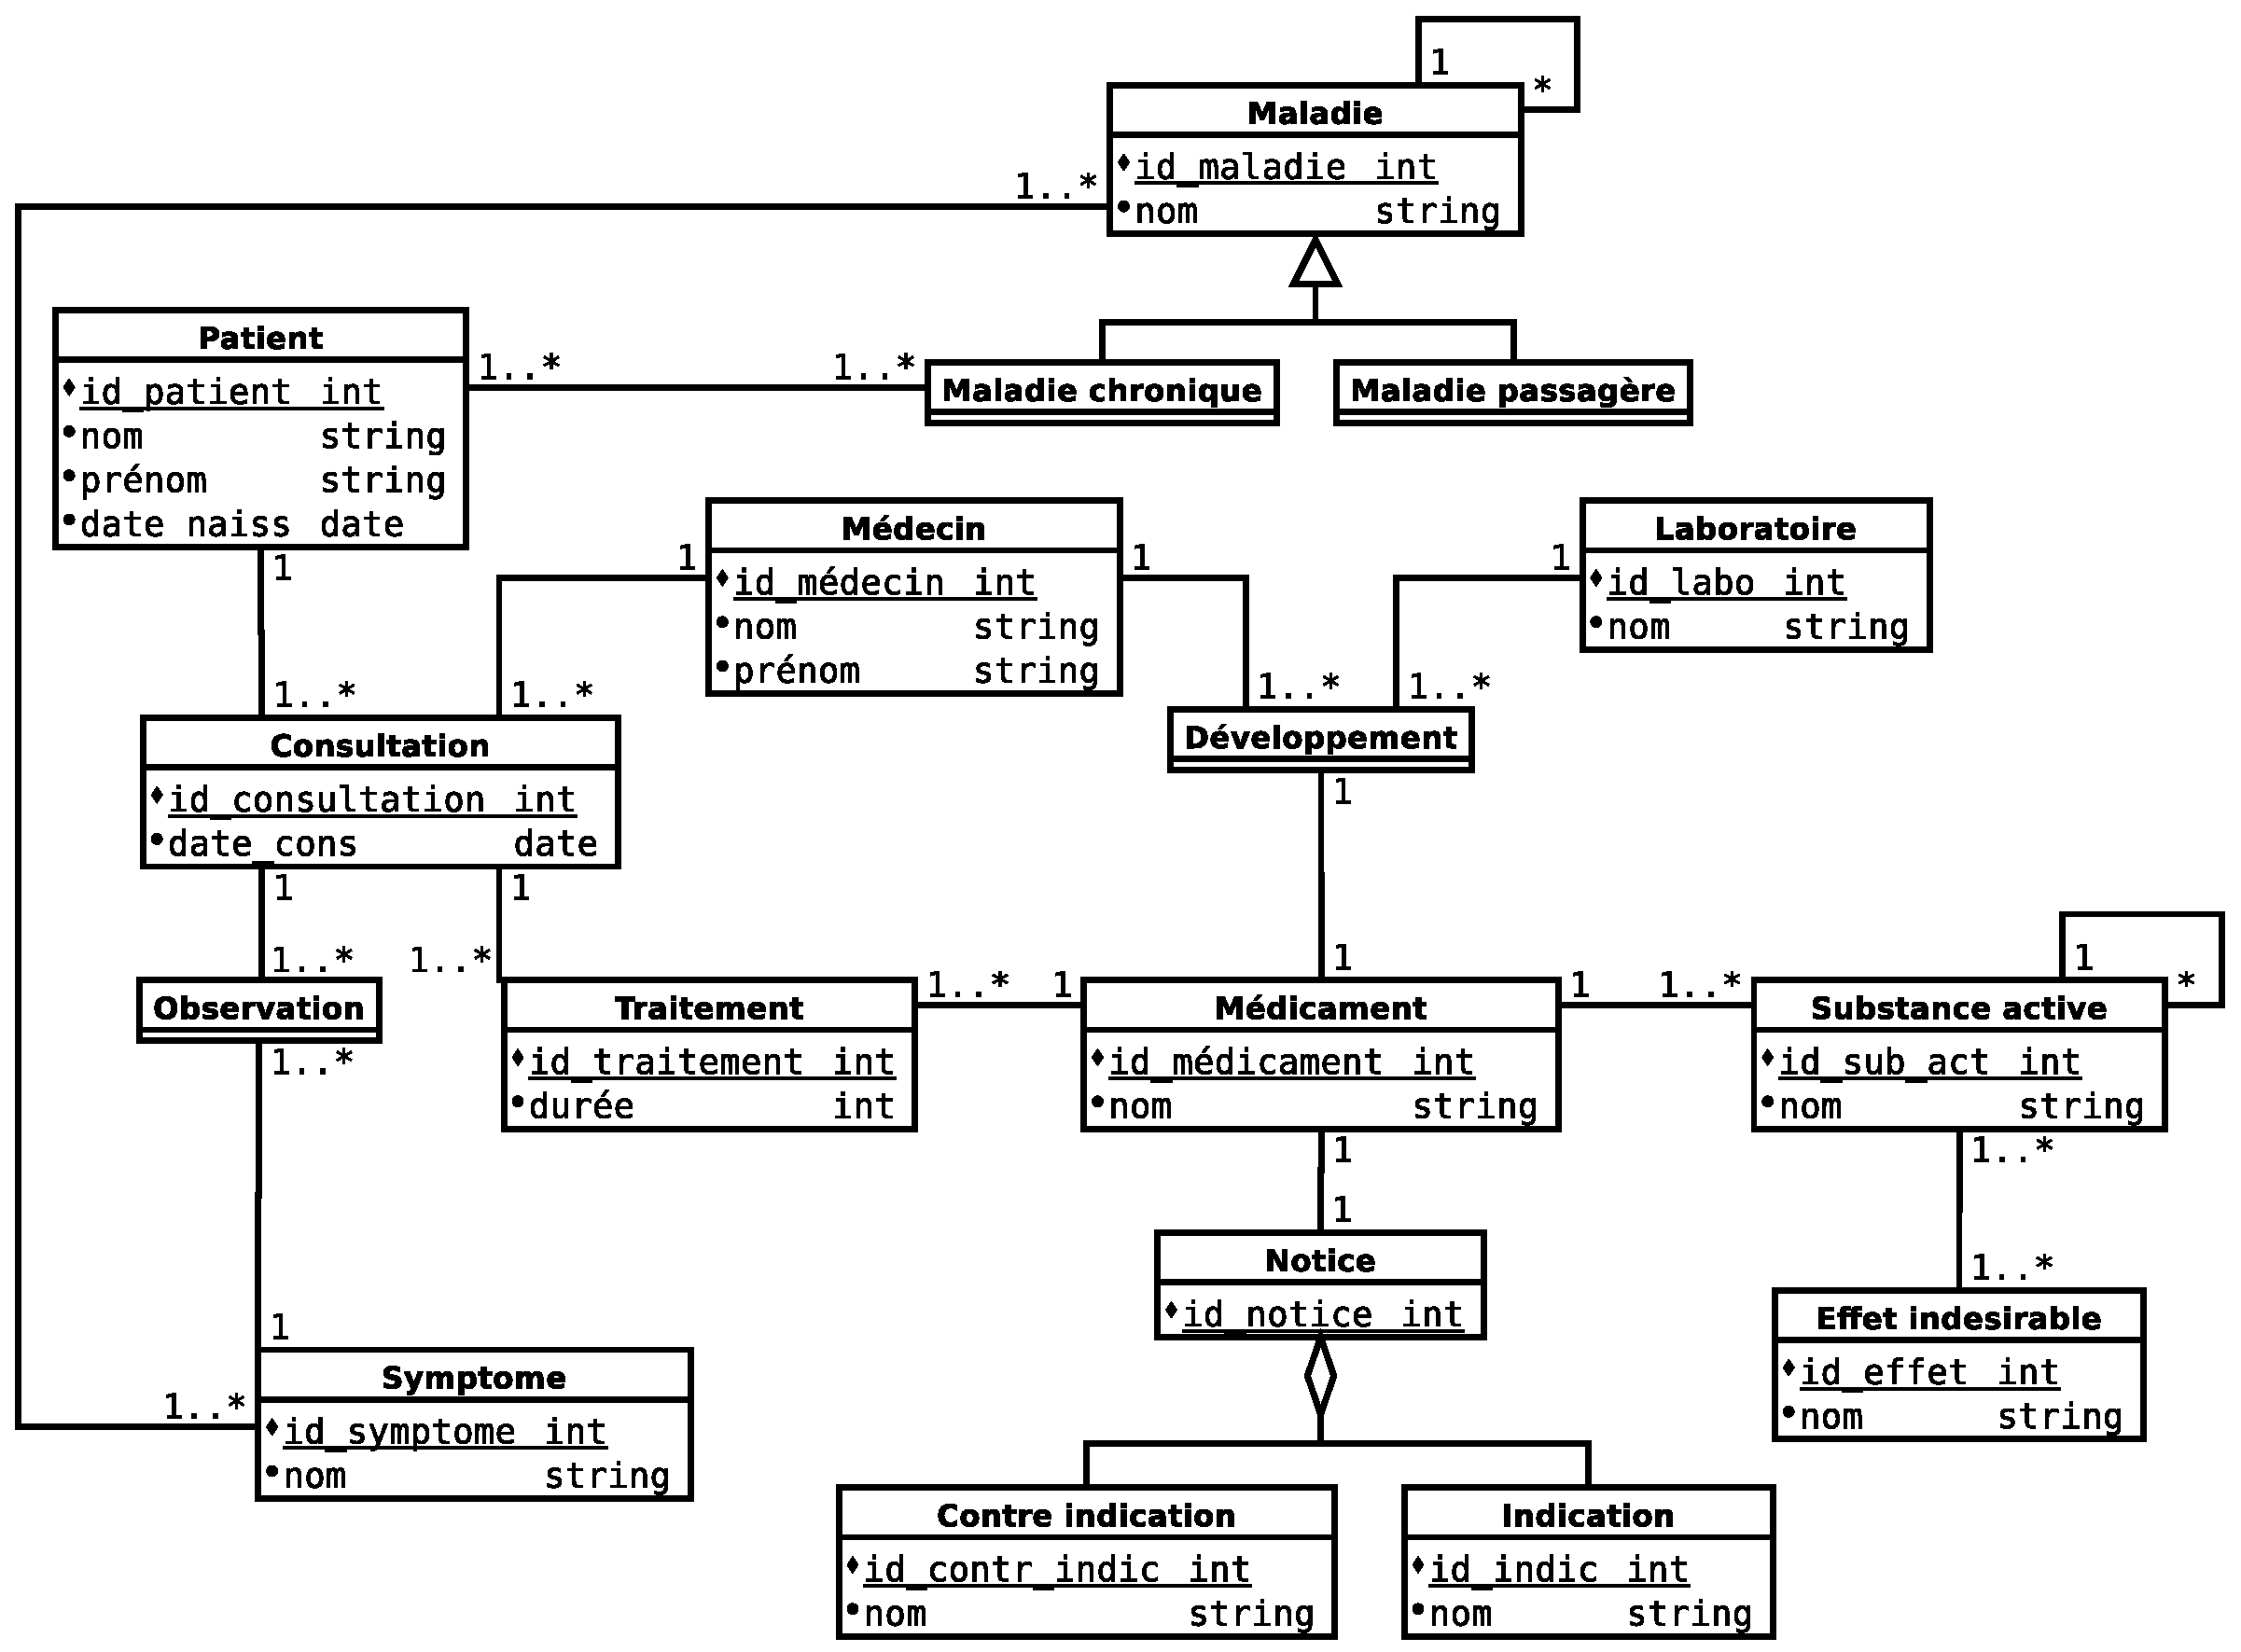
\includegraphics[width=1\linewidth]{er}
	\caption{Diagramme de classes}
	\label{fig:er}
\end{figure}





\subsection{Modèle relationnel}

\subsubsection{Règles de passage au modèle relationnel REF!!!}


\begin{enumerate}
	
	\item Toute classe d'entités du diagramme E/A est représentée par une relation dans le schéma relationnel	équivalent. La clé de cette relation est l'identifiant de la classe
	d'entités correspondante.
	%labels a supprimer
	
	\item Toute classe d'association est transformée en relation. La clé de cette relation est composée de tous les identifiants des entités participantes.
	
	\item Toute classe d'associations reliée à une classe d'entités avec une cardinalité de type 0,1 ou 1,1 peut être fusionnée avec la classe d'entités. Dans ce cas on déplace les attributs de la classe d'associations vers ceux de la relation traduisant la classe d'entités.
	
\end{enumerate}

\subsubsection{Modèle logique des données}

\noindent\textbf{indication} (\underline{id\_indication}, nom\_indication)\\
\textbf{contre\_indication} (\underline{id\_contre\_indic}, nom\_contre\_indic)\\
\textbf{substance\_active} (\underline{id\_sub\_act}, nom\_sub\_act)\\

\noindent\textbf{effet\_indésirable}(\underline{id\_effet}, nom\_effet)\\
\textbf{avoir\_effet}(\underline{id\_sub\_act\#, id\_effet\#})\\
\textbf{notice}(\underline{id\_notice}, indication, contre\_indication, substance\_active)\\
\textbf{laboratoire}(\underline{id\_labo}, nom, adresse)\\
\textbf{médecin}(\underline{id\_médecin}, nom, prénom, adresse)\\
\textbf{médicament}(\underline{id\_médicament}, nom, id\_labo\#, id\_médecin\#, id\_notice\#)\\
\textbf{symptôme}(\underline{id\_symptôme}, nom)\\
\textbf{maladie}(\underline{id\_maladie}, nom)\\
\textbf{avoir\_symptôme}(\underline{id\_symptôme\#, id\_maladie\#})\\
\textbf{consultation}(\underline{id\_patient\# ,id\_médecin\#}, date)\\
\textbf{patient}(\underline{id\_patient}, nom, date\_naissance)\\
\textbf{observation}(\underline{id\_consultation\#, id\_symptôme\#})\\
\textbf{traitement}(durée, \underline{id\_médicament\#, id\_maladie\#})\\
\textbf{recommandation}()


\subsection{Implémentation de la base de données}


Implémentation effectuée sous Oracle-xe-11g shipé dans un conteneur Docker, accessible sur le Docker Hub ainsi que sur Github.




\subsection{Fonctionnalités demandées}

\subsubsection{Sauvegarde des diagnostics et des choix de traitement}
Une méthode prescription qui permettra de sauvegarder le choix de traitement (liste des médicaments) et les maladies diagnostiquées par le médecin pour un patient.
\begin{lstlisting}[frame=single, language=SQL]

\end{lstlisting}




\subsubsection{Traitements en cours}
Une méthode donnant les traitements en cours d’un patient.
\begin{lstlisting}[frame=single, language=SQL]

\end{lstlisting}




\subsubsection{Effets indésirables}
Une méthode donnant la liste et le nombre d’effets indésirables connus d’un médicament.
\begin{lstlisting}[frame=single, language=SQL]
	
\end{lstlisting}



\subsubsection{Médicaments générant des interactions}
Une méthode donnant la liste des médicaments pouvant générer des interactions et l’interaction pour un médicament donné.
\begin{lstlisting}[frame=single, language=SQL]

\end{lstlisting}




\subsubsection{Recommandations à partir d'observations}
Une fonction permettant de proposer une liste de médicaments à partir de la maladie diagnostiquée, même si un lien direct maladie-médicament n’existe
\begin{lstlisting}[frame=single, language=SQL]
	
\end{lstlisting}pas.




\subsubsection{Effets indésirables d'un médicament}
Une méthode qui détermine pour un médicament la liste des effets indésirables probables (déduits des hiérarchies de substances actives).
\begin{lstlisting}[frame=single, language=SQL]

\end{lstlisting}



\subsubsection{Contrôle des prescriptions}
Afin de contrôler les prescriptions, on doit pouvoir déterminer s’il y a un ensemble de médicaments qui ne sont prescrits que par des médecins qui ont travaillé à leur développement.
\begin{lstlisting}[frame=single, language=SQL]

\end{lstlisting}



\subsubsection{}
On doit pouvoir déterminer s’il y a des médicaments qui ne sont prescrits que par des médecins ayant travaillé dans les laboratoires les fabriquant.
\begin{lstlisting}[frame=single, language=SQL]

\end{lstlisting}



\subsubsection{Identification des maladies probables}
On doit pouvoir identifier la/les maladie(s) probable(s) et aider à la prescription en fonction d’observations (symptômes) et des caractéristiques du patient (vous pourrez trier les traitements proposés par nombre d’effets indésirables par exemple).
\begin{lstlisting}[frame=single, language=SQL]

\end{lstlisting}




\subsubsection{Risques d'interaction lors des prescriptions}
Une fonction permettant d’indiquer à un médecin prescrivant si le traitement envisagé, risque d’interagir avec un traitement ’en cours’ et proposer le cas	échéant un autre traitement.
\begin{lstlisting}[frame=single, language=SQL]

\end{lstlisting}




\subsection{Outils Oracle utilisés}

\subsubsection{Tables en ligne ou en colonne et types correspondants}

\textbf{indication\_tpe} et \textbf{contre\_indic\_tpe}  sont des tables en ligne.


\begin{lstlisting}[frame=single, language=SQL]

CREATE TYPE indication_tpe AS TABLE OF indic_type;
/

CREATE TYPE contre_indic_tpe AS TABLE OF contre_indic_type;
/

\end{lstlisting}


\subsubsection{Tables imbriquées}

L'imbrication des tables \textbf{indication} et \textbf{contre\_indication} dans \textbf{notice}.

\begin{lstlisting}[frame=single, language=SQL]

CREATE TABLE notice(id_notice NUMBER(38) CONSTRAINT pk_notice PRIMARY KEY, 
indications     indication_tpe,
contre_indications contre_indic_tpe)
NESTED TABLE indications STORE AS indications_table,
NESTED TABLE contre_indications STORE AS contre_indic_table;

\end{lstlisting}

\subsubsection{Vues}

%la ou il ya SELECT AS

\subsubsection{Séquences}

\subsubsection{Requêtes hiérarchiques}

%Req hierarchique

\subsubsection{Index}

\subsubsection{Triggers}

\subsubsection{Procédures/fonctions}

\subsubsection{PL}

\subsubsection{Curseurs}

\subsubsection{Références}

%rEFERENCES

	
	
	
	
\end{document}
